\documentclass[12pt]{article}

\usepackage{amsmath, amssymb}
\usepackage[right=1.25in,left=1.25in,top=1.1in,bottom=1.1in]{geometry}
\usepackage[round]{natbib}

\usepackage{setspace}
\onehalfspacing
\usepackage{sectsty}

\sectionfont{\large}
\subsectionfont{\normalsize}
\subsubsectionfont{\normalsize}
\usepackage{hyperref}
\hypersetup{colorlinks, citecolor=blue, filecolor=blue, linkcolor=blue, urlcolor=blue}

\usepackage{makecell}
\usepackage{xr}
\usepackage{graphicx}
%\renewcommand{\thesubsection}{\thesection.\alph{subsection}}


\title{Baseline Regression Results}
\author{Luke DiMartino}
\date{April 30, 2022}

\begin{document}

\maketitle

\setcounter{table}{0}
\renewcommand{\tablename}{Appendix Table}
\renewcommand{\figurename}{Appendix Figure}
\renewcommand{\thetable}{A\arabic{table}}
\setcounter{figure}{0}
\renewcommand{\thefigure}{A\arabic{figure}}


\section{Summary}

I am investigating gendered wage gaps in developing India. I am interested in two major aspects of the gaps. First, I am conducting a Machado-Mata decomposition of the wage gap. The MM decomposition builds on the traditional Blinder-Oaxaca decomposition, which splits the difference in means between an advantaged group and a disadvantaged group into a sum of two parts: the difference in endowed characteristics and the difference in returns to those characteristics. For example, men in the United States are on average more educated than women. Knowing only this fact about the two groups, a difference in mean wages is not economically unreasonable --- men are better endowed with characteristics that make them more productive (whether this endowment is systematically unjust or unfair is outside of the scope of this paper). But, men also earn greater returns to these characteristics. For instance, a man experiences greater return for the same graduate degree than a woman. This is economically unreasonable, the so-called "unexplained" part of the gap.

The MM decomposition expands on the Blinder-Oaxaca decomposition by decomposing this gap in a similar manner but at different quantiles of the wage distribution.

I am also interested in the different returns women in particular experience at different quantiles of the wage distribution. As a policymaking tool, this has more obvious implications. Certain covariates may be correlated with higher wages, and causal inference might suggest that in general they raise wages significantly. But, quantile regression allows us to zoom in on certain parts of the distribution to determine whether that effect varies by wage level.


\newpage 

\section{Baseline OLS Results}

\newpage

\begin{table}[!htbp]\centering
\def\sym#1{\ifmmode^{#1}\else\(^{#1}\)\fi}
\caption{\textbf{Pooled OLS Regression Results}}
\small\begin{tabular}{@{\hskip\tabcolsep\extracolsep\fill}l*{4}{c}}
\toprule
                &\multicolumn{1}{c}{\textbf{White SE's}}&\multicolumn{1}{c}{\textbf{Clustered SE's}}&\multicolumn{1}{c}{\textbf{Occupation FE's}}&\multicolumn{1}{c}{\textbf{District FE's}}\\
\midrule
female          &   -0.405\sym{***}&   -0.405\sym{***}&   -0.339\sym{***}&   -0.348\sym{***}\\
                &(0.00491)         &(0.00526)         &(0.00485)         &(0.00465)         \\
\addlinespace
Literacy        &   -0.115\sym{***}&   -0.115\sym{***}&  -0.0500\sym{***}&  -0.0766\sym{***}\\
                &(0.00767)         &(0.00796)         &(0.00727)         &(0.00682)         \\
\addlinespace
Years of Education&   0.0838\sym{***}&   0.0838\sym{***}&   0.0479\sym{***}&   0.0368\sym{***}\\
                &(0.00151)         &(0.00156)         &(0.00146)         &(0.00139)         \\
\addlinespace
Years of Pot. Experience&   0.0335\sym{***}&   0.0335\sym{***}&   0.0239\sym{***}&   0.0158\sym{***}\\
                &(0.00115)         &(0.00117)         &(0.00108)         &(0.00102)         \\
\addlinespace
Marital Status  &   0.0422\sym{***}&   0.0422\sym{***}&   0.0637\sym{***}&   0.0969\sym{***}\\
                &(0.00588)         &(0.00611)         &(0.00558)         &(0.00525)         \\
\addlinespace
Constant        &    2.416\sym{***}&    2.416\sym{***}&    3.586\sym{***}&    4.001\sym{***}\\
                & (0.0160)         & (0.0166)         &  (0.121)         &  (0.124)         \\
\addlinespace
Occupation FE's &       No         &       No         &      Yes         &      Yes         \\
\addlinespace
District FE's   &       No         &       No         &       No         &      Yes         \\
\midrule
Observations    &    93382         &    93382         &    93382         &    93382         \\
Adjusted \(R^{2}\)&    0.364         &    0.364         &    0.444         &    0.520         \\
\textit{AIC}    & 178927.1         & 178927.1         & 166520.3         & 153192.9         \\
\textit{BIC}    & 179078.2         & 179078.2         & 167493.0         & 157782.9         \\
F               &   3013.4         &   2639.6         &    673.4         &    220.3         \\
\bottomrule
\multicolumn{5}{p{\linewidth}}{\footnotesize Standard errors in parentheses}\\
\multicolumn{5}{p{\linewidth}}{\footnotesize All models include caste fixed effects.}\\
\multicolumn{5}{p{\linewidth}}{\footnotesize Additional controls include squared age, indicators for graduate degree holders program income, little english ability, and english fluency.}\\
\multicolumn{5}{p{\linewidth}}{\footnotesize \sym{*} \(p<0.05\), \sym{**} \(p<0.01\), \sym{***} \(p<0.001\)}\\
\end{tabular}
\end{table}


This table is a general ordinary least squares regression on the entire dataset. This table demonstrates a few key results. 

\begin{enumerate}
	\item The naive estimation of the mean wage gap is somewhere between 41\% and 50\%, using exact calculations from the coefficient on female. 
	\item There is not a dramatic difference between White and clustered standard errors. Comparing columns 1 and 2, the standard errors in the second are slightly larger, but not dramatically and not enough to affect results. This is important because although clustered standard errors are theoretically correct, computing them is infeasible for more complex models presented below.
	\item Occupation is a massive source of wage inequality. Controlling for it between columns 2 and 3 absorbs a significant amount of the wage gap.
	\item The coefficient on literacy is negative and statistically significant, suggesting that controlling for all other factors, being literate reduces wages by nearly 8\%. 
\end{enumerate}

\newpage

\begin{table}[htbp]\centering
\def\sym#1{\ifmmode^{#1}\else\(^{#1}\)\fi}
\caption{\textbf{Pooled OLS Subsample Regression Results}}
\begin{tabular}{l*{2}{c}}
\hline\hline
                &\multicolumn{1}{c}{Men}&\multicolumn{1}{c}{Women}\\
\hline
Literacy        &  -0.0564\sym{***}&   -0.101\sym{***}\\
                &(0.00783)         & (0.0142)         \\
[1em]
Years of Education&   0.0203\sym{***}&   0.0192\sym{***}\\
                &(0.00103)         &(0.00228)         \\
[1em]
Marital Status  &    0.111\sym{***}&   0.0133         \\
                &(0.00654)         &(0.00923)         \\
[1em]
Age             &   0.0237\sym{***}&   0.0111\sym{***}\\
                &(0.00104)         &(0.00143)         \\
[1em]
Squared Age     &-0.000220\sym{***}&-0.000101\sym{***}\\
                &(0.0000123)         &(0.0000177)         \\
[1em]
Graduate Degree &    0.224\sym{***}&    0.422\sym{***}\\
                & (0.0212)         & (0.0428)         \\
[1em]
Program Income  &   -0.160\sym{***}&  -0.0712\sym{***}\\
                & (0.0151)         & (0.0135)         \\
[1em]
Little English Ability&   0.0306\sym{***}&   0.0711\sym{***}\\
                &(0.00743)         & (0.0205)         \\
[1em]
English Fluency &    0.184\sym{***}&    0.348\sym{***}\\
                & (0.0148)         & (0.0364)         \\
[1em]
Constant        &    3.824\sym{***}&    3.318\sym{***}\\
                &  (0.132)         &  (0.482)         \\
[1em]
Occupation FE's &      Yes         &      Yes         \\
[1em]
District FE's   &      Yes         &      Yes         \\
\hline
Observations    &    68798         &    26949         \\
Adjusted \(R^{2}\)&    0.478         &    0.463         \\
\textit{AIC}    & 113388.9         &  41596.2         \\
\textit{BIC}    & 117812.1         &  45533.0         \\
F               &    132.4         &        .         \\
\hline\hline
\multicolumn{3}{l}{\footnotesize Standard errors in parentheses}\\
\multicolumn{3}{l}{\footnotesize All models include caste fixed effects.}\\
\multicolumn{3}{l}{\footnotesize \sym{*} \(p<0.05\), \sym{**} \(p<0.01\), \sym{***} \(p<0.001\)}\\
\end{tabular}
\end{table}


This table is a OLS regression on two subsamples, men and women. This is equivalent to using interaction effects with female for every variable, but makes the results a bit more clear. The difference in returns between men and women is considered economically unreasonable, and there are a few variables where this difference is significant. Marital status, in particular, affects men's wages dramatically more than women's, while a graduate degree provides far greater returns to women than to men.

\newpage

\section{Quantile Regression Results}

\begin{figure}
	\centering
	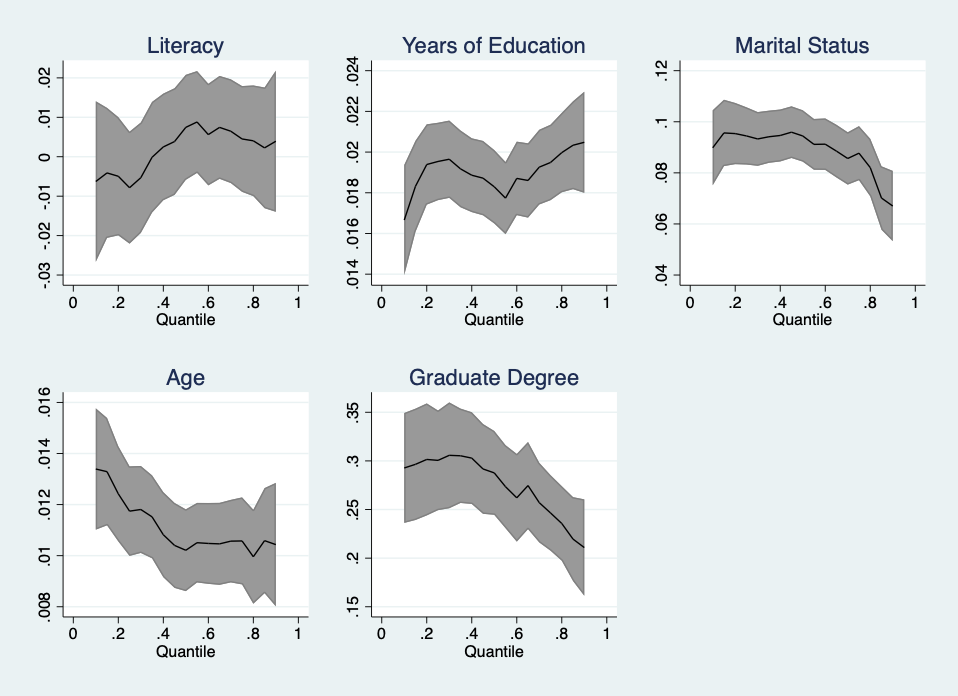
\includegraphics[width=.6\textwidth]{../../paper/figures/full-sample-quantile-coefficients.png}
	\caption{Coefficients from entire sample across quantiles}
\end{figure}

This figure is a model for the main figure I will present in the paper. It shows the estimates of coefficients at different conditional quantiles. However, since this is pretty computationally intensive, this image is from an arbitrary 10\% subsample of the dataset, not from women, which is the figure I will present in the final paper.

\begin{figure}
	\centering
	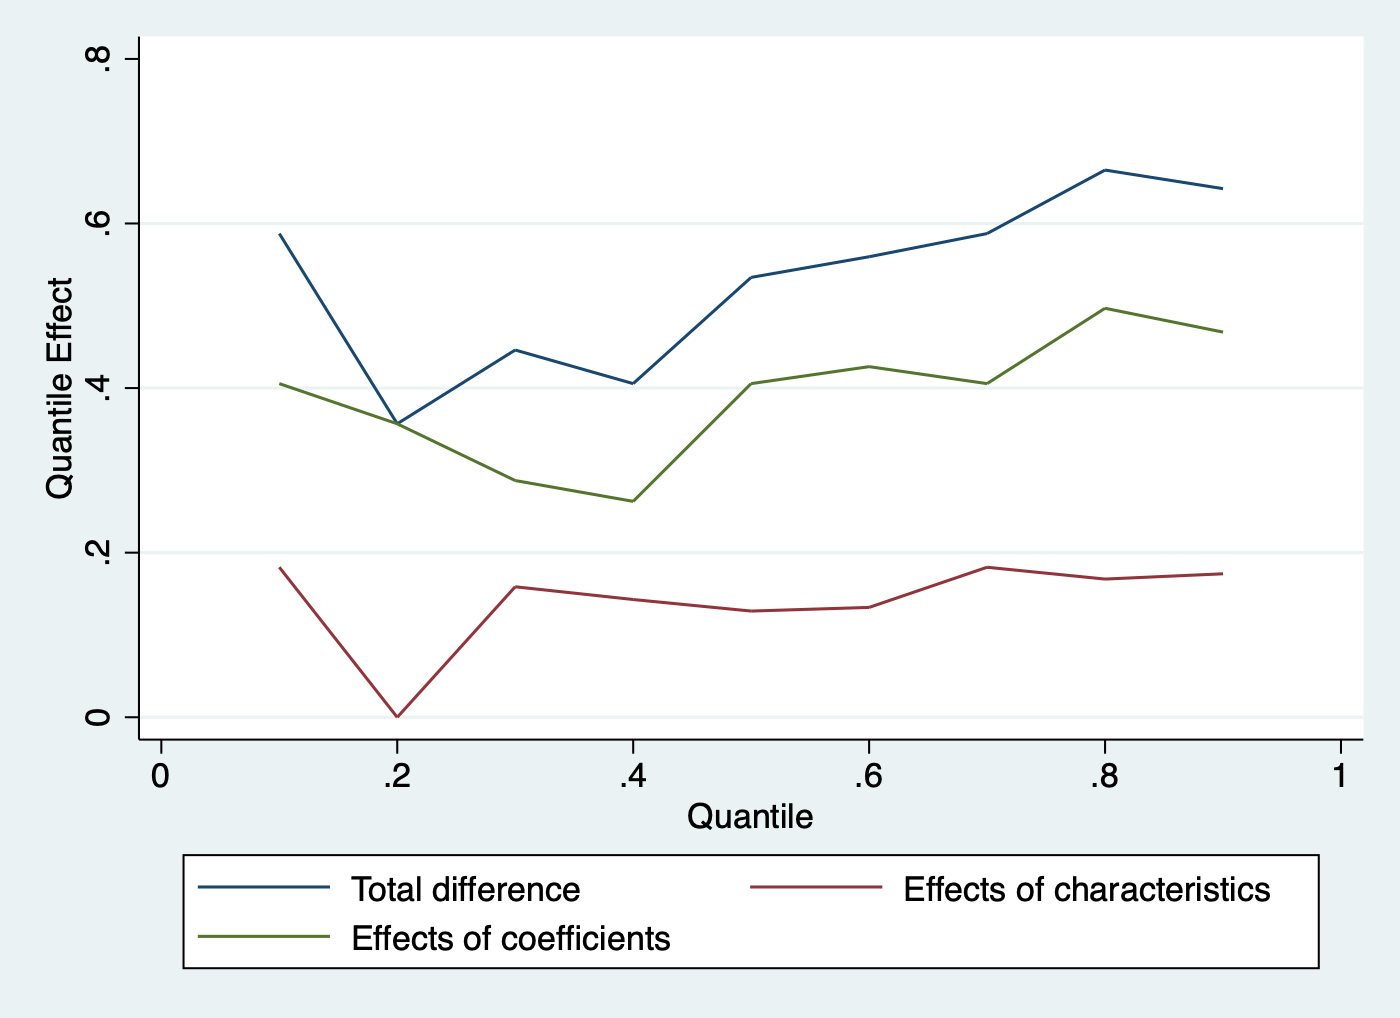
\includegraphics[width=.6\textwidth]{../../paper/figures/mm-decomp.png}
	\caption{Decomposition of wage gap across quantiles}
\end{figure}	

This figure shows the decomposition of the wage gap by decile. The second decile suggests a problem in the estimation procedure --- I am working on this. The "effects of coefficients" are the effects of greater returns, while the "effects of characteristics" are the effect on the wage gape cause by differing endowments.

\begin{figure}
	\centering
	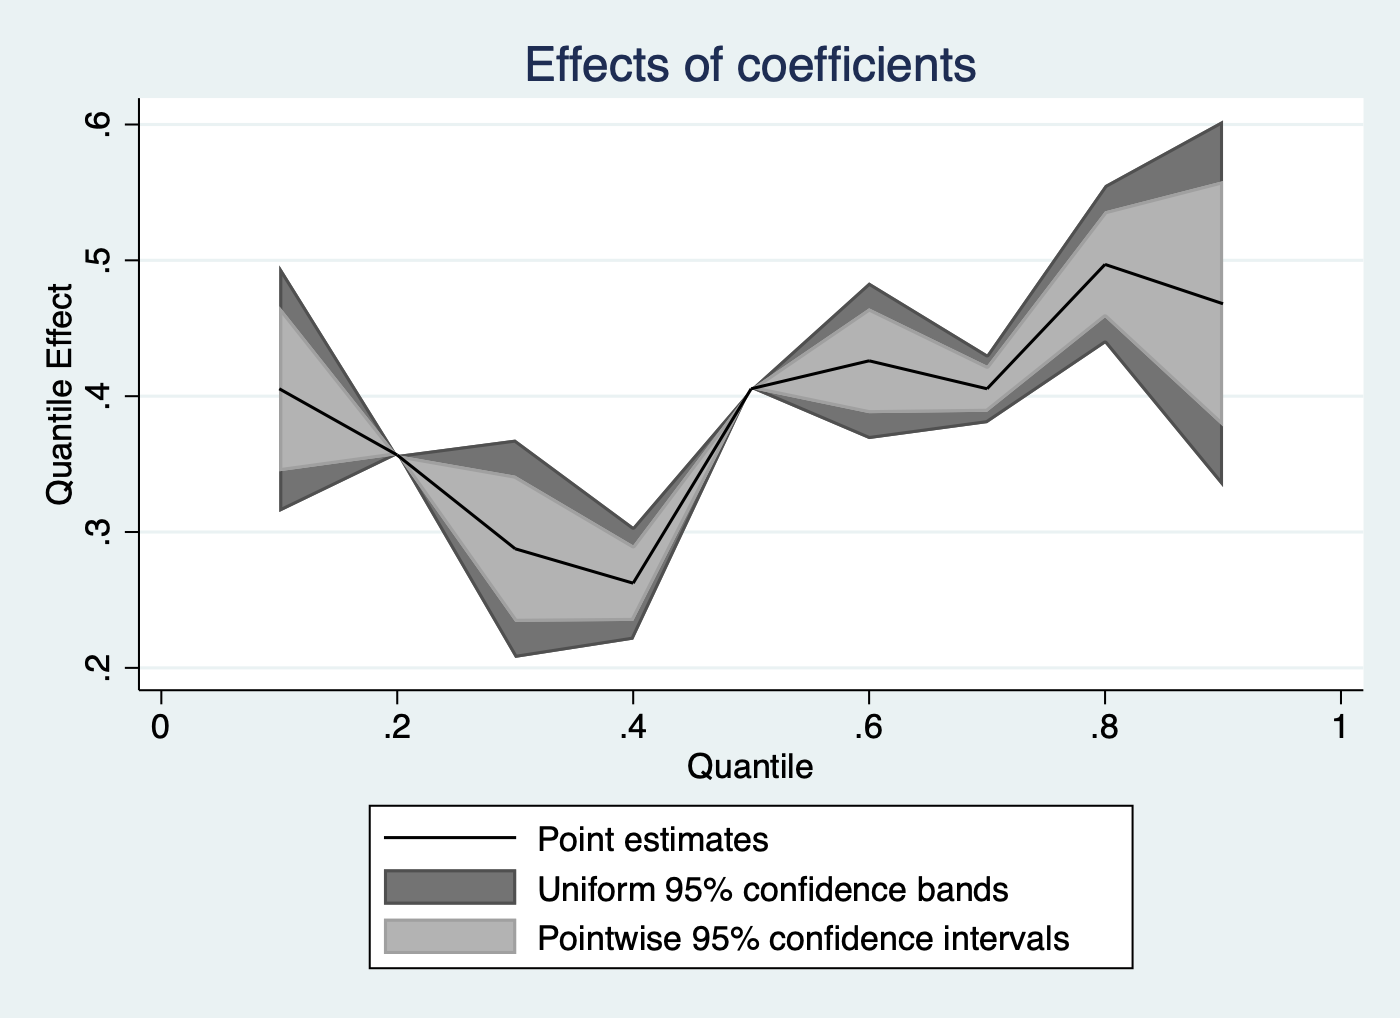
\includegraphics[width=.6\textwidth]{../../paper/figures/mm-coef-effects.png}
	\caption{Confidence interval around coefficient effect across quantiles}
\end{figure}	

\section{Moving Forward}

Moving forward, I would like to potentially add more control variables and fine-tune the more complex models.

\end{document}

